
\documentclass[letterpaper,hide notes,xcolor={table,svgnames},pdftex]{beamer}
\def\showexamples{t}


%\usepackage[svgnames]{xcolor}

%% Demo talk
%\documentclass[letterpaper,notes=show]{beamer}

\usecolortheme{crane}
\setbeamertemplate{navigation symbols}{}

\usetheme{MyPittsburgh}
%\usetheme{Frankfurt}

%\usepackage{tipa}

\usepackage{hyperref}
\usepackage{graphicx,xspace}
\usepackage[normalem]{ulem}

\newcommand\SF[1]{$\bigstar$\footnote{SF: #1}}



\newcounter{tmpnumSlide}
\newcounter{tmpnumNote}

% old question code
%\newcommand\question[1]{{$\bigstar$ \small \onlySlide{2}{#1}}}
% \newcommand\nquestion[1]{\ifdefined \presentationonly \textcircled{?} \fi \note{\par{\Large \textbf{?}} #1}}
% \newcommand\nanswer[1]{\note{\par{\Large \textbf{A}} #1}}


 \newcommand\mnote[1]{%
   \addtocounter{tmpnumSlide}{1}
   \ifdefined\showcues {~\tiny\fbox{\arabic{tmpnumSlide}}}\fi
   \note{\setlength{\parskip}{1ex}\addtocounter{tmpnumNote}{1}\textbf{\Large \arabic{tmpnumNote}:} {#1\par}}}

\newcommand\mmnote[1]{\note{\setlength{\parskip}{1ex}#1\par}}

%\newcommand\mnote[2][]{\ifdefined\handoutwithnotes {~\tiny\fbox{#1}}\fi
% \note{\setlength{\parskip}{1ex}\textbf{\Large #1:} #2\par}}

%\newcommand\mnote[2][]{{\tiny\fbox{#1}} \note{\setlength{\parskip}{1ex}\textbf{\Large #1:} #2\par}}

\newcommand\mquestion[2]{{~\color{red}\fbox{?}}\note{\setlength{\parskip}{1ex}\par{\Large \textbf{?}} #1} \note{\setlength{\parskip}{1ex}\par{\Large \textbf{A}} #2\par}\ifdefined \presentationonly \pause \fi}

\newcommand\blackboard[1]{%
\ifdefined   \showblackboard
  {#1}
  \else {\begin{center} \fbox{\colorbox{blue!30}{%
         \begin{minipage}{.95\linewidth}%
           \hspace{\stretch{1}} Some space intentionally left blank; done at the blackboard.%
         \end{minipage}}}\end{center}}%
         \fi%
}



%\newcommand\q{\tikz \node[thick,color=black,shape=circle]{?};}
%\newcommand\q{\ifdefined \presentationonly \textcircled{?} \fi}

\usepackage{listings}
\lstset{%
  keywordstyle=\bfseries,
  aboveskip=15pt,
  belowskip=15pt,
  captionpos=b,
  identifierstyle=\ttfamily,
  escapeinside={(*@}{@*)},
  stringstyle=\ttfamiliy,
  frame=lines,
  numbers=left, basicstyle=\scriptsize, numberstyle=\tiny, stepnumber=0, numbersep=2pt}

\usepackage{siunitx}
\newcommand\sius[1]{\num[group-separator = {,}]{#1}\si{\micro\second}}
\newcommand\sims[1]{\num[group-separator = {,}]{#1}\si{\milli\second}}
\newcommand\sins[1]{\num[group-separator = {,}]{#1}\si{\nano\second}}
\sisetup{group-separator = {,}, group-digits = true}

%% -------------------- tikz --------------------
\usepackage{tikz}
\usetikzlibrary{positioning}
\usetikzlibrary{arrows,backgrounds,automata,decorations.shapes,decorations.pathmorphing,decorations.markings,decorations.text}

\tikzstyle{place}=[circle,draw=blue!50,fill=blue!20,thick, inner sep=0pt,minimum size=6mm]
\tikzstyle{transition}=[rectangle,draw=black!50,fill=black!20,thick, inner sep=0pt,minimum size=4mm]

\tikzstyle{block}=[rectangle,draw=black, thick, inner sep=5pt]
\tikzstyle{bullet}=[circle,draw=black, fill=black, thin, inner sep=2pt]

\tikzstyle{pre}=[<-,shorten <=1pt,>=stealth',semithick]
\tikzstyle{post}=[->,shorten >=1pt,>=stealth',semithick]
\tikzstyle{bi}=[<->,shorten >=1pt,shorten <=1pt, >=stealth',semithick]

\tikzstyle{mut}=[-,>=stealth',semithick]

\tikzstyle{treereset}=[dashed,->, shorten >=1pt,>=stealth',thin]

\usepackage{ifmtarg}
\usepackage{xifthen}
\makeatletter
% new counter to now which frame it is within the sequence
\newcounter{multiframecounter}
% initialize buffer for previously used frame title
\gdef\lastframetitle{\textit{undefined}}
% new environment for a multi-frame
\newenvironment{multiframe}[1][]{%
\ifthenelse{\isempty{#1}}{%
% if no frame title was set via optional parameter,
% only increase sequence counter by 1
\addtocounter{multiframecounter}{1}%
}{%
% new frame title has been provided, thus
% reset sequence counter to 1 and buffer frame title for later use
\setcounter{multiframecounter}{1}%
\gdef\lastframetitle{#1}%
}%
% start conventional frame environment and
% automatically set frame title followed by sequence counter
\begin{frame}%
\frametitle{\lastframetitle~{\normalfont(\arabic{multiframecounter})}}%
}{%
\end{frame}%
}
\makeatother

\makeatletter
\newdimen\tu@tmpa%
\newdimen\ydiffl%
\newdimen\xdiffl%
\newcommand\ydiff[2]{%
    \coordinate (tmpnamea) at (#1);%
    \coordinate (tmpnameb) at (#2);%
    \pgfextracty{\tu@tmpa}{\pgfpointanchor{tmpnamea}{center}}%
    \pgfextracty{\ydiffl}{\pgfpointanchor{tmpnameb}{center}}%
    \advance\ydiffl by -\tu@tmpa%
}
\newcommand\xdiff[2]{%
    \coordinate (tmpnamea) at (#1);%
    \coordinate (tmpnameb) at (#2);%
    \pgfextractx{\tu@tmpa}{\pgfpointanchor{tmpnamea}{center}}%
    \pgfextractx{\xdiffl}{\pgfpointanchor{tmpnameb}{center}}%
    \advance\xdiffl by -\tu@tmpa%
}
\makeatother
\newcommand{\copyrightbox}[3][r]{%
\begin{tikzpicture}%
\node[inner sep=0pt,minimum size=2em](ciimage){#2};
\usefont{OT1}{phv}{n}{n}\fontsize{4}{4}\selectfont
\ydiff{ciimage.south}{ciimage.north}
\xdiff{ciimage.west}{ciimage.east}
\ifthenelse{\equal{#1}{r}}{%
\node[inner sep=0pt,right=1ex of ciimage.south east,anchor=north west,rotate=90]%
{\raggedleft\color{black!50}\parbox{\the\ydiffl}{\raggedright{}#3}};%
}{%
\ifthenelse{\equal{#1}{l}}{%
\node[inner sep=0pt,right=1ex of ciimage.south west,anchor=south west,rotate=90]%
{\raggedleft\color{black!50}\parbox{\the\ydiffl}{\raggedright{}#3}};%
}{%
\node[inner sep=0pt,below=1ex of ciimage.south west,anchor=north west]%
{\raggedleft\color{black!50}\parbox{\the\xdiffl}{\raggedright{}#3}};%
}
}
\end{tikzpicture}
}


%% --------------------

%\usepackage[excludeor]{everyhook}
%\PushPreHook{par}{\setbox0=\lastbox\llap{MUH}}\box0}

%\vspace*{\stretch{1}

%\setbox0=\lastbox \llap{\textbullet\enskip}\box0}

\setlength{\parskip}{\fill}

\newcommand\noskips{\setlength{\parskip}{1ex}}
\newcommand\doskips{\setlength{\parskip}{\fill}}

\newcommand\xx{\par\vspace*{\stretch{1}}\par}
\newcommand\xxs{\par\vspace*{2ex}\par}
\newcommand\tuple[1]{\langle #1 \rangle}
\newcommand\code[1]{{\sf \footnotesize #1}}
\newcommand\ex[1]{\uline{Example:} \ifdefined \presentationonly \pause \fi
  \ifdefined\showexamples#1\xspace\else{\uline{\hspace*{2cm}}}\fi}

\newcommand\ceil[1]{\lceil #1 \rceil}


\AtBeginSection[]
{
   \begin{frame}
       \frametitle{Outline}
       \tableofcontents[currentsection]
   \end{frame}
}



\pgfdeclarelayer{edgelayer}
\pgfdeclarelayer{nodelayer}
\pgfsetlayers{edgelayer,nodelayer,main}

\tikzstyle{none}=[inner sep=0pt]
\tikzstyle{rn}=[circle,fill=Red,draw=Black,line width=0.8 pt]
\tikzstyle{gn}=[circle,fill=Lime,draw=Black,line width=0.8 pt]
\tikzstyle{yn}=[circle,fill=Yellow,draw=Black,line width=0.8 pt]
\tikzstyle{empty}=[circle,fill=White,draw=Black]
\tikzstyle{bw} = [rectangle, draw, fill=blue!20, 
    text width=4em, text centered, rounded corners, minimum height=2em]
    
    \newcommand{\CcNote}[1]{% longname
	This work is licensed under the \textit{Creative Commons #1 3.0 License}.%
}
\newcommand{\CcImageBy}[1]{%
	\includegraphics[scale=#1]{creative_commons/cc_by_30.pdf}%
}
\newcommand{\CcImageSa}[1]{%
	\includegraphics[scale=#1]{creative_commons/cc_sa_30.pdf}%
}
\newcommand{\CcImageNc}[1]{%
	\includegraphics[scale=#1]{creative_commons/cc_nc_30.pdf}%
}
\newcommand{\CcGroupBySa}[2]{% zoom, gap
	\CcImageBy{#1}\hspace*{#2}\CcImageNc{#1}\hspace*{#2}\CcImageSa{#1}%
}
\newcommand{\CcLongnameByNcSa}{Attribution-NonCommercial-ShareAlike}

\newenvironment{changemargin}[1]{% 
  \begin{list}{}{% 
    \setlength{\topsep}{0pt}% 
    \setlength{\leftmargin}{#1}% 
    \setlength{\rightmargin}{1em}
    \setlength{\listparindent}{\parindent}% 
    \setlength{\itemindent}{\parindent}% 
    \setlength{\parsep}{\parskip}% 
  }% 
  \item[]}{\end{list}} 




\usepackage{alltt}

\title{Lecture 6 --- Events, Polling vs. Interrupts}

\author{Patrick Lam \& Jeff Zarnett \\ \small \texttt{p.lam@ece.uwaterloo.ca} \& \texttt{jzarnett@uwaterloo.ca}}
\institute{Department of Electrical and Computer Engineering \\[-1ex]
  University of Waterloo}
\date{\today}


\begin{document}


\begin{frame}
  \titlepage

\end{frame}

\begin{frame}
\frametitle{Goal}

\Large

\begin{changemargin}{2.5cm}
Be able to program for systems which use event-based models (eg Android).
\end{changemargin}

\end{frame}


\begin{frame}
\frametitle{Random Request}

\begin{changemargin}{2.5cm}
In 10 minutes, please remind me that I'm supposed to do something.
\end{changemargin}

\end{frame}

\begin{frame}
\frametitle{Relevance of OO to Android: Events}

\begin{changemargin}{1.5cm}
What happens when you press this?

\begin{center}

\includegraphics{images/go-button}
\end{center}
\large \uncover<2>{Android sends an \alert{event} to the \alert{event listener}.}
\end{changemargin}

\end{frame}

\begin{frame}
\frametitle{Events}

\begin{changemargin}{2.5cm}
\Large
An \emph{event} is a notification of a change to the state of your system.
\end{changemargin}

\end{frame}

\begin{frame}
\frametitle{About event-based programming}

\begin{changemargin}{2.5cm}
\begin{itemize}
\Large Reactive, not proactive.
\end{itemize}
\end{changemargin}

\end{frame}

\begin{frame}
\frametitle{Event Listeners}

\begin{changemargin}{1.5cm}
\begin{itemize}
\item To receive click events: \\
\begin{changemargin}{1em}
the application registers an event 
listener with the object representing the button.\\
\uncover<2>{\tt \qquad go.setOnClickListener(\ldots);}
\end{changemargin}
\item When the user clicks the button: \\
\begin{changemargin}{1em}
the system executes the click event listener.
\end{changemargin}
\end{itemize}
\end{changemargin}

\end{frame}


\begin{frame}[fragile]
\frametitle{Implementing Event Listeners (painfully)}

\begin{changemargin}{1.5cm}
We need to pass something to {\tt setOnClickListener()}. What?\\[1em]

This method takes a {\tt View.OnClickListener} object.\\[1em]

You could declare one:

{\small
\begin{verbatim}
class MyClickListener 
      extends View.OnClickListener {
  public void onClick(View v) {
    Log.d("A2", "clicked!");
  }
}

...
go.setOnClickListener(new MyClickListener()); 
\end{verbatim}
}

\end{changemargin}

\end{frame}

\begin{frame}[fragile]
\frametitle{A Better Way}

\begin{changemargin}{1.5cm}

{\small
\begin{verbatim}
go.setOnClickListener(new View.OnClickListener() {
  public void onClick(View v) {
    Log.d("A2", "clicked!");
  }
  }); 
\end{verbatim}
}

{\Large This is called an \alert{inner class}.}

\end{changemargin}
\end{frame}

\begin{frame}[fragile]
\frametitle{Advantages of Inner Classes}

{\small
\begin{verbatim}
class MainActivity {
  int i;

  @Override
  protected void onCreate(Bundle savedInstanceState) {
    Button go = (Button) findViewById(R.id.go);
    final int j = 2;
    go.setOnClickListener(new View.OnClickListener() {
      public void onClick(View v) {
        Log.d("A2", "i is "+i+" and j is "+j);
      }
      }); 
  }
}
\end{verbatim}
}

\begin{changemargin}{1.5cm}
\begin{itemize}
\item They don't litter your code with one-time-use classes.
\item They can access fields and (final) local variables.
\end{itemize}
\end{changemargin}

\end{frame}

\begin{frame}[fragile]
\frametitle{Alternative to Inner Classes}

\begin{changemargin}{1cm}
You have another option. From the Android documentation\footnote{\tiny \url{http://developer.android.com/reference/android/widget/Button.html}}:
\begin{verbatim}
  <Button
     android:layout_height="wrap_content"
     android:layout_width="wrap_content"
     android:text="@string/self_destruct"
     android:onClick="selfDestruct" />
\end{verbatim}
~\\[1em]

Then, in your activity, you must include the method:
\begin{verbatim}
  public void selfDestruct(View view) {
     // Kabloey
  }
\end{verbatim}
\end{changemargin}

\end{frame}

\begin{frame}
\frametitle{Callback methods}

\begin{changemargin}{2.5cm}
We've been programming with \alert{callback methods}.\vfill
This is also known as ``inversion of control''.\vfill
Key idea: system (user) decides what happens when.
\end{changemargin}

\end{frame}

\begin{frame}
\frametitle{Leveraging callback methods}

\begin{changemargin}{1.5cm}
You can also structure your program with callback methods.
Say you have a time-consuming task (TCT).\vfill
\begin{enumerate}
\item register a callback upon completion of TCT;
\item spawn the TCT in another thread, don't wait for it;
\item continue normally.
\end{enumerate}\vfill
Once the TCT finishes, the callback notifies the main application,
which collects results.\vfill
Also known as asynchronous, or non-blocking, execution.
\end{changemargin}

\end{frame}

\begin{frame}
\frametitle{Synchronous versus Asynchronous Execution}

\begin{changemargin}{1cm}
ECE150: Synchronous, or sequential, programs:
\begin{itemize}
\item all instructions execute in sequence;
\item an instruction only executes after its predecessor completes.
\end{itemize}
Also true for function calls.\\[1em]

ECE155, ECE254: Asynchronous, or concurrent, programs:
\begin{itemize}
\item most instructions execute in sequence; but
\item main program may spawn a function to run concurrently with it.
\item Communication via shared memory or via events.
\end{itemize}
Permits higher performance on multicores, or more relevant structuring.
Callbacks are a tool.
\end{changemargin}

\end{frame}

\begin{frame}
\frametitle{Events}

\Large

\begin{changemargin}{1cm}
Where do events come from?
\end{changemargin}

\end{frame}

\begin{frame}
\frametitle{Digression: Priorities}

\begin{changemargin}{1cm}
Imagine the following situation:
\begin{itemize}
\item your mom calls;
\item supper is burning;
\item laundry is done.
\end{itemize}

What do you do?
\end{changemargin}

\end{frame}

\begin{frame}
\frametitle{Implementing Priorities}

\begin{changemargin}{1cm}
Associate a priority with each event.

Use a \emph{priority queue} data structure to get the highest-priority event.
\end{changemargin}

\begin{center}

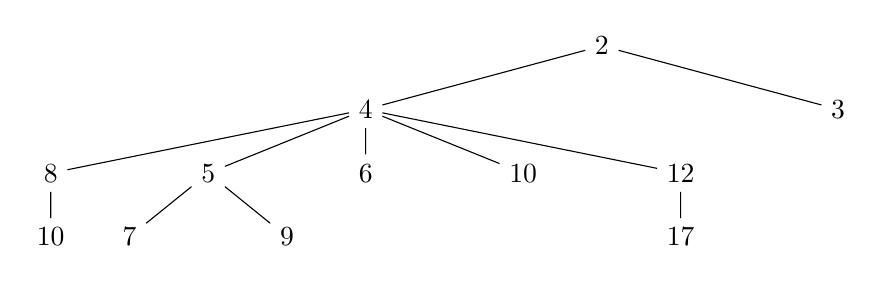
\begin{tikzpicture}[level 1/.style={sibling distance=60mm}, level 2/.style={sibling distance=20mm}, level distance=2.3em]
\node (2) {2}
  child {node (4) {4} %[sibling distance=20mm]
     child {node {8} child { node {10}}}
     child {node {5} child { node {7} } child { node {9}}}
     child {node {6} }
     child {node {10}}
     child {node {12} child { node {17}}}}
  child {node {3} };
\end{tikzpicture}
\end{center}
\end{frame}

\begin{frame}
\frametitle{Events and Finite-State Machines}

\begin{changemargin}{1cm}
Remember: reactive, not proactive.\vfill
How can the application do what it wants?\vfill
\Large Use \alert{Finite-State Machines}!
\end{changemargin}

\uncover<2>{
\begin{center}
\scalebox{0.6}{
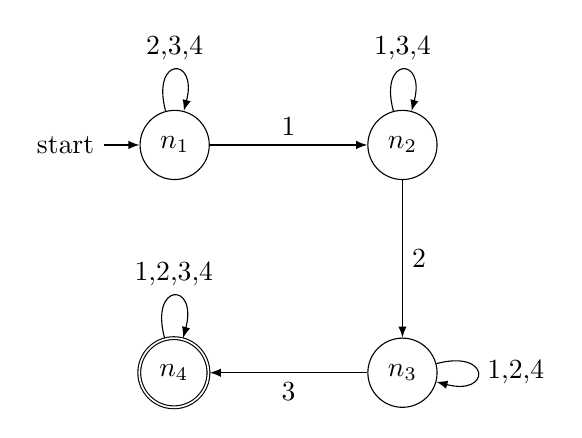
\begin{tikzpicture} [node distance=2cm, auto, every loop/.style={-latex},  every initial by arrow/.style={-latex}]

\node [state, initial] 	(n0){$n_1$};
\node [state] 			(n1) [right=of n0,]	{$n_2$};
\node [state]			(n2) [below=of n1]	{$n_3$};
\node [state, accepting](n3) [left=of n2]	{$n_4$};

\path[-latex] 
		(n0)edge				node	{1}		(n1)
			edge [loop above]	node	{2,3,4}	()
		(n1)edge				node	{2}		(n2)
			edge [loop above]	node	{1,3,4}	()
		(n2)edge				node	{3}		(n3)
			edge [loop right]	node	{1,2,4}	()
		(n3)edge [loop above]	node	{1,2,3,4}()
		;


\end{tikzpicture}}
\end{center}
}


\end{frame}

\begin{frame}
\frametitle{Where Events Come From}

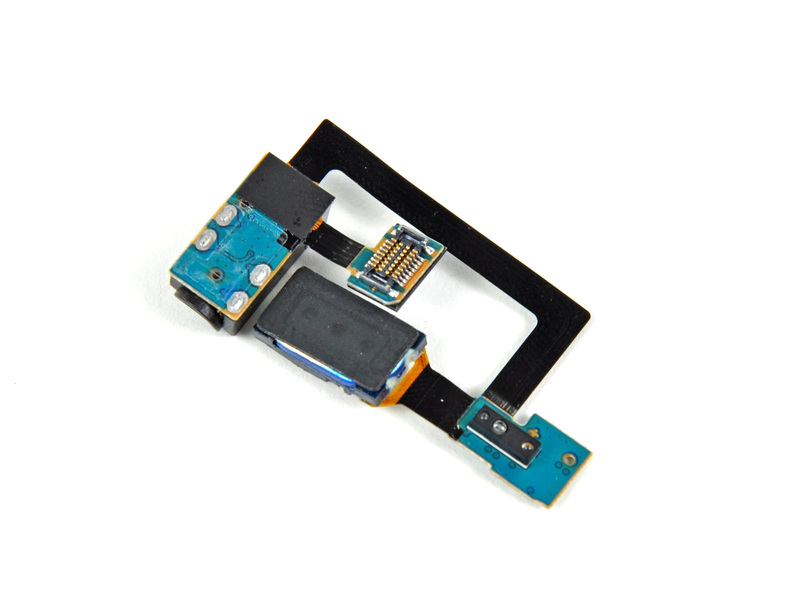
\includegraphics[width=.9\textwidth]{images/Galaxy_S_4G_037-small.jpg}

\vspace*{-1em}
\uncover<2>{Analog-to-Digital Converter. Then what?}

\end{frame}

\begin{frame}

\Huge
\begin{center}
``Are we there yet?''
\end{center}

\uncover<2>{\hfill --- example of \alert{polling}.}

\end{frame}

\begin{frame}
\frametitle{Polling}

\Large
\begin{changemargin}{2cm}
Polling: processor requests readings from
the device at its convenience.  \vfill
``What is the current light level?''\vfill
(also known as ``passive synchronization'')
\end{changemargin}

\end{frame}

\begin{frame}
\frametitle{When to Poll?}

\large
\begin{changemargin}{2cm}
It depends:

\begin{itemize}
\item whenever convenient (occasional polling);
\item at fixed time intervals (periodic polling); or
\item constantly (tight polling).
\end{itemize}
\end{changemargin}

\end{frame}

\begin{frame}
\frametitle{How to Get the Data}

\begin{center}
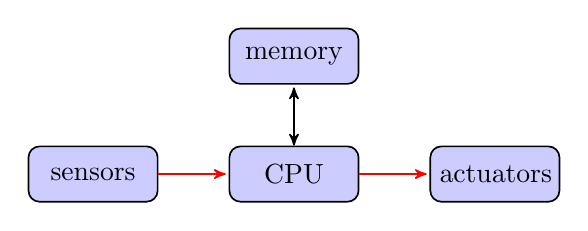
\begin{tikzpicture}[->,>=stealth',shorten >=1pt,auto,node distance=2.2cm,
                    semithick,initial text=]
  \node[bw]   (cpu)               {CPU};
  \node[bw, left of=cpu,xshift=-1em] (sensors) {sensors};
  \node[bw, right of=cpu,xshift=1em] (actuators) {actuators};
  \node[bw, above of=cpu,yshift=-2em] (memory) {memory};

  \path (cpu) edge[<->] node {} (memory)
        (sensors) edge[red] node {} (cpu)
        (cpu) edge[red] node {} (actuators);
\end{tikzpicture}
\end{center}

\large 
\begin{changemargin}{2cm} \vspace*{1em} What's the mechanism?

\uncover<2>{
\begin{itemize}
\item port-mapped I/O; or,\\[0.5em]
\item memory-mapped I/O
\end{itemize}
}
\end{changemargin}


\end{frame}

\begin{frame}[fragile]
\frametitle{Port-mapped I/O: Special CPU Instructions}

\begin{changemargin}{1.5cm}
The Intel ia32 processors provide special I/O instructions:\\[1em]
\begin{verbatim}
    outb   ax, 0x3f8
    inw    dx, ax
\end{verbatim}
~\\
May use a special bus, or set a specific signal on the bus.
\end{changemargin}

\end{frame}


\begin{frame}
\frametitle{Memory-mapped I/O Example}

\begin{changemargin}{1cm}
CPU just reads and writes to ``memory''.\\[1em]
\end{changemargin}

\small
\begin{changemargin}{1em}
\begin{alltt}
 while (\alert{statusRegister} == 0x0000) \{\\
 \qquad // Do nothing until statusRegister changes value\\
 \}\\
 //  Read data that has changed from a dataRegister\\
 //  and store in memory\\
 incomingData = \alert{dataRegister};\\
\end{alltt}
\end{changemargin}

\begin{changemargin}{1cm}
~\\[1em] Devices listen on the bus and respond.
\end{changemargin}


\end{frame}

\begin{frame}
\frametitle{Memory-mapped I/O Example}

\small
\begin{changemargin}{1em}
\begin{alltt}
 while (\alert{statusRegister} == 0x0000) \{\\
 \qquad // Do nothing until statusRegister changes value\\
 \}\\
 //  Read data that has changed from a dataRegister\\
 //  and store in memory\\
 incomingData = \alert{dataRegister};\\
\end{alltt}
\end{changemargin}

\begin{changemargin}{1.5cm}
This is a \emph{tight polling loop}.\\[1em]
\begin{itemize}
\item Expect the hardware specification to promise that statusRegister eventually changes 
due to an external event.
\item Data exchange occurs once device is ready: \alert{polling synchronization}.
\end{itemize}
\end{changemargin}


\end{frame}

\begin{frame}
\frametitle{Interrupts: an alternative to polling}

\large
\begin{changemargin}{1cm}
So far: processor controls when to read data from a device.\vfill
Instead: device may tell the processor when device is ready,
using an \alert{interrupt}.\vfill
This constitutes \alert{active synchronization}.
\end{changemargin}

\end{frame}

\begin{frame}
\frametitle{How Interrupts Work}

\begin{changemargin}{1cm}
Interrupt tells the processor: ``Something's happening!''\vfill

Upon receipt of an interrupt, the processor:
\begin{itemize}
\item stops what it's currently doing and saves its state;
\item starts executing pre-defined \alert{interrupt handler}, which:
\begin{itemize}
\item reads the event information; and
\item stores it somewhere accessible.
\end{itemize}
\item upon return from handler, resumes previous state.
\end{itemize}
\end{changemargin}

\end{frame}

\begin{frame}
\frametitle{Inversion of Control: Without It}

\begin{changemargin}{1cm}
Old ECE150 paradigm:\\[2em]

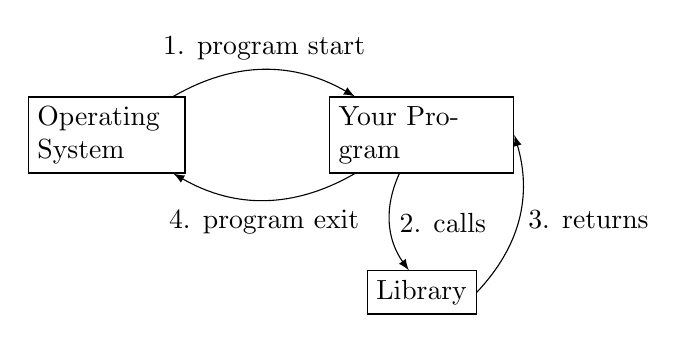
\begin{tikzpicture}
\path (0, 0) node[draw,text width=5em] (OS) { Operating System }
    +(4, 0) node[draw, text width=6em] (you) {Your Program};
\path<2-4> (4, -2) node[draw] (lib) {Library};

\path[->,bend left,>=latex] (OS) edge node[above] {1. program start} (you);
\path<4>[->,bend left,>=latex] (you) edge node[below] {4. program exit} (OS);
\path<2->[->,bend right,>=latex] (you) edge node[right] {2. calls} (lib);
\path<3->[->,bend right,>=latex] (lib.east) edge node[right] {3. returns} (you.east);
\end{tikzpicture}

\end{changemargin}

\end{frame}

\begin{frame}
\frametitle{Inversion of Control: With It}

\begin{changemargin}{1cm}
New event-driven ECE155 paradigm:\\[2em]

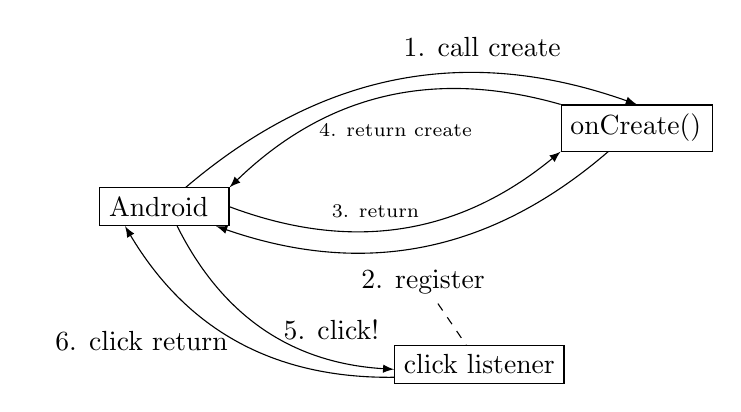
\begin{tikzpicture}
\path (0, 0) node[draw,text width=4em] (OS) { Android }
    +(6, 1) node[draw, text width=4.8em] (you) { onCreate() };
\path<2-> (4, -2) node[draw] (listener) {click listener};

\path[->,bend left,>=latex] (OS) edge node[above,yshift=0.5em, xshift=3em] {1. call create} (you.north);
\path<2->[->,bend left,>=latex] (you) edge node[below,name=reg,yshift=-.5em] {2. register} (OS);
\path<2->[dashed] (reg) edge (listener);
\path<3->[<-,bend left,>=latex] (you.south west) edge node[above,xshift=-1em,name=reg] {\scriptsize 3. return} (OS.east);
\path<4->[->,bend right,>=latex] (you.north west) edge node[above,at end,xshift=6em,yshift=1.5em] {\scriptsize 4. return create} (OS.north east);
\path<5->[->,bend right,>=latex] (OS) edge node[right] {~5. click!} (listener);
\path<6->[<-,bend right,>=latex] (OS.south)+(-0.5,0) edge node[left] {~~6. click return} 
                                 (listener)+(1,0);
\end{tikzpicture}

\end{changemargin}

\end{frame}

\begin{frame}[fragile]
\frametitle{Behind the Scenes for Inversion of Control}

\begin{changemargin}{1cm}
Android is running an event loop for each thread:


\begin{verbatim}
while (!done) {
 r <- fetch Runnable from Queue
 dispatch r
}
\end{verbatim}

This is a polling loop: in particular, a \structure{tight polling loop}, but which
goes to sleep waiting for the next event (in fetch).
\end{changemargin}

\end{frame}

\begin{frame}
\frametitle{Miscellaneous: Real-Time Systems}

\begin{changemargin}{1cm}
Must respond to an external event in a fixed amount of time. \\[1em]

This fixed amount of time is not necessarily small.
\begin{itemize}
\item may potentially be fixed and large.
\end{itemize}

Many embedded systems must satisfy real-time constraints.\\[1em]

In upper-year courses, you'll see both embedded systems and real-time
systems in more detail.
\end{changemargin}

\end{frame}

\begin{frame}
\frametitle{Real-Time System Example}

\begin{center}
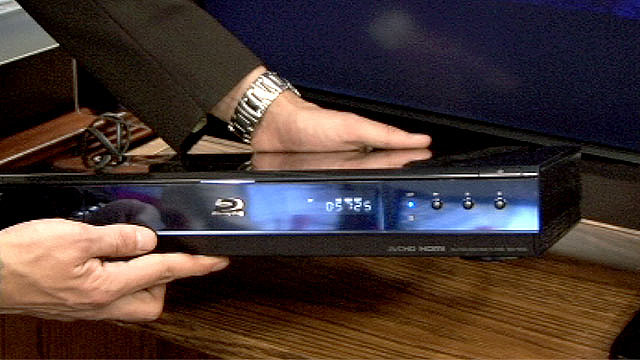
\includegraphics[width=.6\textwidth]{images/bluray}
\end{center}
\hfill {\small (credit {\tt digitaljournal.com}, from flickr)}

\begin{changemargin}{1cm}
Blu-Ray player must:
\begin{itemize}
\item read compressed video data from a media disk;
\item decompress the video; and
\item output it to a HDMI interface,
\end{itemize}
all within a fixed amount of time, to avoid a degradation of video quality.
\end{changemargin}

\end{frame}



\end{document}

